\chapter{Protocolo de Autenticação e Autorização proposto}\label{cap:Protocolo}

%A Polícia Civil do Distrito Federal, diante da necessidade de compartilhar suas informações com órgão parceiros, no intuito de possibilitar que os sistemas possam ser integrados de forma eficiente e principalmente segura busca estabelecer uma arquitetura de referência para a adoção de uma arquitetura orientada a serviços. Essa arquitetura deve primar pela segurança, haja vista a criticidade e sensibilidade das informações que são tratadas no âmbito da PCDF.

%Dessa forma, optou-se por adotar a tecnologia de Web Services usando o protocolo REST para implementar SOA na instituição. Neste caso, estudos específicos foram realizados com vistas a estabelecer uma política de segurança eficiente que possibilite o fornecimento dos serviços e promova a integração com os órgãos parceiros.

A Polícia Civil do Distrito Federal, diante da necessidade de compartilhar suas informações com órgão parceiros, de forma eficiente e segura, 
objetiva estabelecer uma arquitetura de referência para a adoção de uma arquitetura orientada a servi\c cos. Essa arquitetura deve primar pela segurança, 
dada a criticidade e sensibilidade das informações que são tratadas no âmbito da PCDF ({\color{red}conforme discutido no Cap\'{i}tulo~\ref{}}).
Dessa forma, optou-se pela ado\c c\~{a}o de uma solu\c c\~{a}o {\color{red}baseada no modelo \emph{REST}} para implementar uma arquitetura orientada a servi\c cos 
na instituição. Neste cen\'{a}rio, essa disserta\c c\~{a}o contribui com um protocolo de autenticação e autorização que atende às 
necessidades particulares da PCDF, mas que tamb\'{e}m pode ser adotado em outras institui\c c\~{o}es. {\color{red}Este cap\'{i}tulo inicia com a apresenta\c c\~{a}o 
dos requisitos do protocolo, \ldots}.

\section{Requisitos do Protocolo}\label{sec:reqprotocolo}

Conforme discutido, o protocolo de autenticação e autorização deve ser aderente a arquitetura REST ({\color{blue}importante discutir o porqu\^{e} da escolha por REST, em algum ponto do documento}), de forma a permitir que os serviços ofertados pela Divisão de Tecnologia possam ser acessados por um número relativamente grande de clientes {\color{red}\'{e} isso mesmo?}. 
Os requisitos inerentes ao protocolo são descritos nesta seção.

\begin{enumerate}[RQ1]

\item Segurança de sessão. Toda comunicação entre o cliente e o servidor deve ser realizada utilizando HTTPS 
\emph{(Hypertext Transfer Protocol over Secure Sockets Layer)}, usando o SSL/TLS para garantir a confidencialidade 
e integridade para a sessão. Para isso será usado o certificado digital X.509, emitido por uma autoridade de certificação, 
para encriptar as comunicações e garantir a autenticidade do servidor e do cliente. Os clientes devem realizar a validação do 
certificado antes de interagir com o servidor.

\item Seguran\c ca na troca de mensagens. Deve ser utilizada criptografia assimétrica {\color{red} em quais situa\c c\~{o}es?} 
para promover a segurança na troca de mensagens realizada entre o Cliente e a PCDF. 
Todas as mensagens deverão ser assinadas digitalmente. Para isso, será utilizado uma função HASH, com o algoritmo SHA (Secure Hash Algorithm).

\item Autoriza\c c\~{a}o e escalabildiade. O protocolo deve permitir acesso aos serviços apenas ao pessoal {\color{red}pessoal ou institui\c c\~{o}es} 
autorizado, de forma que a autenticação e autorização siga os padrões definidos na política de segurança. Para ser autenticado e autorizado, o usuário 
deve apresentar credenciais válidas. Essas credenciais devem ser criptografadas, assinadas e enviadas no cabeçalho do protocolo HTTPS. 
Devendo ser escalável em termos de sobrecarga, tamanho do domínio de proteção e de manutenção. Além disso, ele deverá permitir a 
preservação de privacidade, uma vez que para proteger os clientes e fornecedores de recursos de entidades maliciosas, suas interações 
deverão revelar o mínimo de informações possíveis. {\color{red}quem deve ser escalado, quem \'{e} ``ele'' anteriormente. 
Reescrever. Os requisitos nesse par\'{a}grafo est\~{a}o bem misturados.} 

\item Flexibilidade. A autenticação e autorização deve ser baseada em desafios e resposta, que serão elaborados a partir da apresentação de declarações de identidade (\emph{Claims}). Tal requisito torna mais flexível o gerenciamento da identidade do usuário, uma vez que possibilita ao administrador desabilitar credenciais que tenham sido comprometidas de forma transparente ao usuário.

\item Contratos previamente definidos. A política de autenticação e autorização 
proposta no protocolo será estabelecida por meio de contratos, onde serão definidos 
todas as regras que deverão ser atendidas pelos usuário e pelo fornecedor do serviço.

\end{enumerate}

Dessa forma, para que qualquer usu\'{a}rio {\color{red}(usuário ou insitui\c c\~{a}o)} 
possa ter acesso aos serviços ofertados pela Divisão de Tecnologia da PCDF, 
faz-se necess\'{a}rio o estabelecimento de um contrato prévio de acesso. Ou seja, 
primeiramente devem ser estabelecidos as restri\c c\~{o}es de acesso e autorização. 
Uma vez cadastrado, o {\color{red}usuário ou institui\c c\~{a}o} deve 
informar as credenciais para comprovar a identidade no momento da autenticação, 
de forma que ele possa ser autorizado de acordo com o seus {\color{red}privilégios ou permiss\~{o}es}.

No momento do estabelecimento do contrato, ser\~{a}o geradas 
para o cliente múltiplas credenciais, que devem ser utilizadas no processo de autenticação e 
autorização. Essas informações 
devem ser compartilhados entre o Cliente, o \servidorAA{} e o \servidorRest{} 
({\color{red}esses n\'{o}s processadores j\'{a} foram introduzidos?}). 
Além disso, o Contrato poderá ter acesso a múltiplos serviços. A Figura ~\ref{fig:diagrama_relacionamento} apresenta o relacionamento entre o contrato, as credenciais e os serviços.

\begin{figure}[!htb]
    \centering
    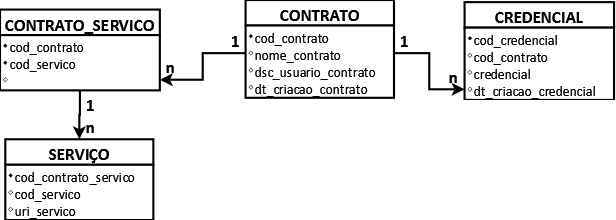
\includegraphics[width=0.8\textwidth]{modelo_relacionamento_contrato1.png}
    \caption{Diagrama de relacionamento entre contrato, credenciais e usuários}
    \label{fig:diagrama_relacionamento}
\end{figure}


%Para a implementação de segurança em aplicações REST, verificou-se que ela passa basicamente pela aplicação de segurança em protocolos \emph{HTTP}, que oferece dois tipos de autenticação:  \emph{Basic} e \emph{Digest}.

%A autenticação Basic é um modelo baseado no desafio e resposta, sendo utilizada por servidores HTTP para validar a autenticação~\cite{franks1999}. Desta forma, quando o cliente tenta acessar algum recurso protegido, a sua identidade é requerida pelo servidor, o cliente então fornece a resposta codificada em base64 no header \emph{HTTP},  se a resposta for correta ela terá acesso ao sistema. Porém, por não criptografar o desafio, estando esse apenas codificado, faz com que ele seja vulnerável e sujeito a ataques, como por exemplo, os de repetição.

%Já na Digest, o processo é o mesmo que na autenticação básica. Sendo que seu mecanismo de autenticação é um pouco mais complexo, uma vez que ele gera um HASH, geralmente utilizando o algoritmo MD5, do desafio que será enviado pelo servidor ao cliente ~\cite{franks1999}. Apesar de ser mais seguro do que a autenticação básica, autenticação HTTP Digest também é vulnerável à ataques, como por exemplo o man-in-the-middle.  Para evitar esse problema, deve ser empregado a segurança na camada de transporte~\cite{Webber10}.

\section{Arquitetura do Protoloco}\label{sec:ArqProtocolo}

A arquitetura do protocolo proposto é apresentada na Figura~\ref{fig:arquiteturaprotocolo}. O protocolo é composto por quatro componentes: Cliente, 
\servidorAA, \servidorRest, e \servidorBD--- que gerencia contratos, credenciais e \emph{tokens} de acesso.

\begin{figure}[!htb]
    \centering
    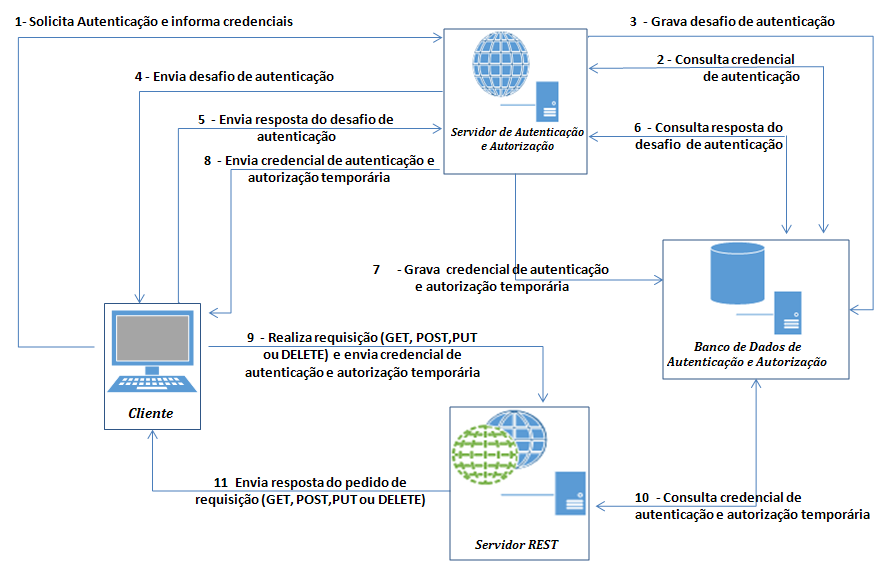
\includegraphics[width=0.8\textwidth]{arquitetura_protocolo.png}
    \caption{Fluxo do protocolo de autenticação/autorização proposto, 1º cenário.}
    \label{fig:arquiteturaprotocolo}
\end{figure}

O componente Cliente na arquitetura do protocolo representa as Instituições ou Órgãos conveniados, que após firmar um contrato, podem consumir os serviços ofertados pela PCDF.
O Servidor de Autenticação e Autorização tem um papel fundamental na arquitetura do protocolo, pois é nele que o gerenciamento de autenticação e autorização é realizado. Desta forma, o servidor de Autenticação e Autorização é responsável por realizar os processos de verificação e validação de credenciais, criação dos desafios de autenticação, criação de \emph{tokens} JSON e a criação e o gerenciamento das credenciais de autenticação e autorização temporárias, que são utilizados pelos clientes para consumir os serviços requisitados.
O Servidor de Fachada REST atua como uma fachada, abstraindo toda lógica necessária para o consumo dos serviços. Neste servidor estão concentrados os serviços REST disponibilizados pela PCDF. Desta forma, quando um Cliente necessita acessar um serviço, primeiramente ele deve ser autenticado e autorizado no servidor de Autenticação e Autorização. Após esse processo, o Cliente faz a requisição ao servidor de Fachada REST, que realiza as verificações necessárias para saber se o Cliente tem privilégios ou não para acessar o serviço. {\color{red}Ele (evitar, quem \'{e} ``ele'')} O servidor de Fachada REST acessa a base de dados de Autenticação e Autorização para confirmar as credenciais de autenticação e autorização temporária informadas e, caso elas sejam válidas, permite que o Cliente acesse o serviço requerido. Um ponto importante a ser destacado é que os desenvolvedores, ao desenvolver um serviço, não necessitam ter preocupações de segurança, uma vez que é esse componente que realiza {\color{red}esse atividade (que atividade???)}. Finalmente, o servidor de Banco de Dados mant\'{e}m as informa\c c\~{o}es necess\'{a}rias   para o funcionamento dos serviços de autenticação e autorização. É neste servidor que são salvas os usuários, os desafios e as credenciais de autorização e autenticação temporária.


\subsection{Visão geral do protocolo de Autenticação e Autorização proposto}

Para ter acesso a API \emph{REST}, referente aos serviços ofertados, o cliente deve ser autenticado e autorizado a acessar o serviço. Para isso, o protocolo usa a autenticação baseada em \emph{tokens} de segurança, que são recipientes de reivindicações da autoridade emissora. Os \emph{tokens} de segurança utilizados (\emph{Web Tokens}) seguem o formato \emph{JSON}. Esse formato, ao contrário dos tokens \emph{SAML}, que são baseados em \emph{XML}, são mais compactos e, portanto, mais adequados para serem usados em um cabeçalho \emph{HTTP}. Além disso, todas as mensagens do protocolo s\~{a}o assinadas e criptografadas de forma assimétrica. O processo de autenticação e autorização é descrito em dois cenários distintos. No primeiro cenário, representado na Figura~\ref{fig:protocoloseguro}, o Cliente não está autenticado. No segundo cenário, o Cliente está autenticado e possui uma 
credencial de autorização. %Esse último é representado na figura ~\ref{fig:cenario2}.

\subsubsection{Primeiro cenário}

No primeiro cenário, o Cliente não está autenticado e deve solicitar a autenticação pela primeira vez, conforme descrito a seguir:

\begin{figure}[!htb]
    \centering
    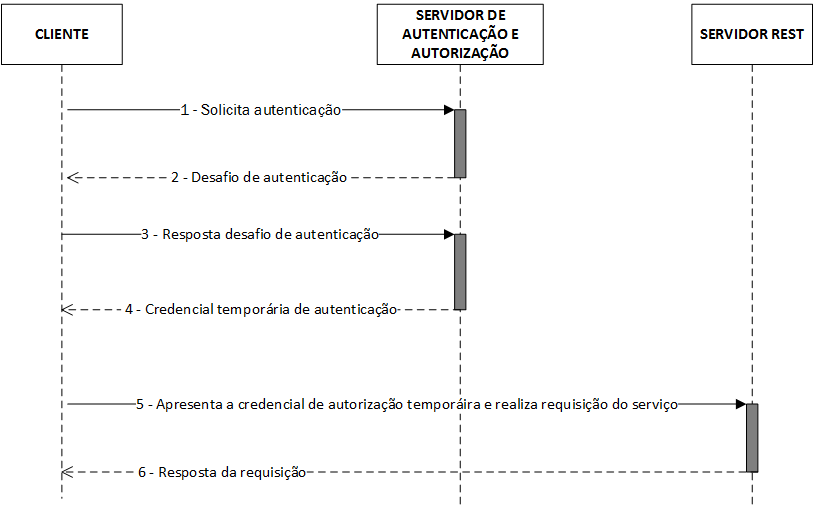
\includegraphics[width=1.0\textwidth]{fluxo_autenticacao.png}
    \caption{Fluxo do protocolo de autenticação/autorização proposto, 1º cenário.}
    \label{fig:protocoloseguro}
\end{figure}


O protocolo tem início quando o Cliente envia uma solicitação de autenticação ao \servidorAA.
Esse pedido é realizado por meio de uma mensagem (mensagem 1 da Figura~\ref{fig:protocoloseguro}) 
que contém um \emph{token} JSON, enviado no cabeçalho HTTP da requisição REST. O \emph{token} contém uma 
credencial, extraída de forma aleatória da tabela de credenciais do Cliente. O token é assinado digitalmente pelo Cliente 
e cifrado com a chave pública do \servidorAA. É importante frisar que tanto o Cliente quanto o 
\servidorAA{} possuem as mesmas tabelas de credenciais e de serviços, pois elas são 
geradas no momento de assinatura do contrato de prestação do serviço.

Na segunda mensagem, ao receber uma solicitação de autenticação, o \servidorAA{} extrai o 
token cifrado com sua chave privada e verifica a autenticidade e integridade da requisição por meio da verificação da assinatura digital do Cliente.  
Se houver qualquer problema, o c\'{o}digo HTTP 401 (usuário não autorizado) é retornada ao Cliente.
Tamb\'{e}m \'{e} feita a verifica\c c\~{a}o de \emph{timestamp}, que se refere ao tempo de envio da mensagem. Caso a mensagem tenha 
sido enviada em um período de tempo superior ao pré-estabelecido no contrato, o Cliente recebe 
como resposta o c\'{o}digo HTTP {\color{red}adicionar o c\'{o}digo} (usuário não autenticado). {\color{red}importante padronizar a escrita}

Caso não ocorram problemas, procede-se com o processo de validação da credencial informada. Tal processo consiste em 
consultar a credencial em uma base de dados e verificar se a credencial \'{e} válida e associada ao Cliente. Em seguida, o \servidorAA{} 
gera um desafio de autenticação. Tal desafio consiste em fazer uma busca aleatória à tabela de credenciais e selecionar um código de 
credencial que esteja associado ao Cliente. Em seguida, os dados relacionados ao desafio, a data e hora de geração do desafio e a resposta que o Cliente deverá 
fornecer s\~{a}o persistidos no \servidorBD. Finalmente, o \emph{token} JSON, contendo o código do desafio, o código da credencial e um \emph{timestamp} representando a data e hora de criação do desafio é enviado ao Cliente. Tal \emph{token} \'{e} assinado digitalmente pelo \servidorAA{} \'{e} cifrado com a chave pública do 
Cliente que está solicitando a autenticação.

Na terceira mensagem, após receber o desafio do \servidorAA, o Cliente extrai o token cifrado com sua chave 
privada e verifica a autenticidade e integridade da requisição por meio da verificação da assinatura digital do \servidorAA. 
Em seguida {\color{red}quem considera?} considera o \emph{timestamp} com o objetivo de verificar se a mensagem foi 
enviada em um período de tempo superior ao pré-estabelecido no contrato. Se for detectada alguma inconsist\^{e}ncia, 
o processo de autenticação atual é descartado e inicia-se um novo processo de autenticação.

Caso nenhuma inconsist\^{e}ncia seja identificada, o Cliente verifica e responde o desafio solicitado, enviando-o 
juntamente com um \emph{timestamp} e o código do serviço que deseja consumir, para o \servidorAA{} 
por meio de um \emph{token} JSON, que é assinado digitalmente pelo Cliente e cifrado com a chave pública do \servidorAA.

Na quarta mensagem, o \servidorAA{} recebe a resposta do desafio de autenticação, decifra o token e verifica a autenticidade e integridade 
da requisição por meio da verificação da assinatura digital do Cliente.  Não ocorrendo nenhuma viola\c c\~{a}o, inicia-se o processo de 
verificação da resposta. A primeira verificação realizada refere-se ao tempo de geração do desafio, por meio do \emph{timestamp}. Se a resposta 
tiver sido enviada em um período de tempo superior ao pré-estabelecido em contrato, o \servidorAA{} responde com o 
c\'{o}digo HTTP 401 (usuário não autorizado). Caso contrário, {\color{red}esses ``eles'' deixam muita margem de d\'{u}vidas. diria que esse \'{e} o 
problema de escrita mais recorrente.} \sout{ele} procede com a verificação do desafio que consiste em realizar uma consulta na tabela de desafios 
verificando se a resposta ao desafio corresponde a esperada. Caso a resposta esteja correta o \servidorAA{} 
autentica o Cliente. Em seguida o \servidorAA{} verifica, considerando o código do serviço requisitado, 
se o Cliente tem privilégios necessários para consumir o serviço requisitado.

Caso o Cliente possua os privil\'{e}gios necess\'{a}rios, o \servidorAA{} gera uma credencial de autenticação e autorização temporária para o serviço solicitado. Tal 
credencial é gravada em uma tabela de credencias de autorização temporária, juntamente com a data e hora de criação, a 
data de expiração e o código do cliente. A tabela de credencias de autorização temporária \'{e} posteriormente acessada pelo \servidorRest{}  
para verificar quais privilégios o Cliente tem acesso e se o mesmo está autenticada. O \emph{token}, contendo a credencial de 
autenticação e autorização temporária, é  assinado digitalmente pelo \servidorAA{} e cifrado  com a chave pública do Cliente. 
Após esse processo, o \emph{token} é enviado ao Cliente.

Caso a resposta do desafio esteja em desacordo com a esperada ou se o Cliente não tiver privilégios 
suficientes para acessar o serviço requisitado, a resposta do \servidorAA{} cont\'{e}m o c\'{o}digo HTTP 401 (usuário não autorizado).
É importante destacar que a credencial de autenticação e autorização temporária será gerada apenas para o serviço que o Cliente tenha 
solicitado e possua o privilégio de acesso para utilizá-la. Nesse caso, a credencial 
será válida por um período  de tempo que será definido no momento da assinatura do contrato de prestação de serviço, 
entre o órgão conveniado e a PCDF.

Na quinta mensagem, o Cliente, extrai o \emph{token} cifrado com sua chave privada e verifica a autenticidade e integridade 
da requisição por meio da verificação da assinatura digital do \servidorAA. Em seguida consulta  
o \emph{timestamp} para verificar se a mensagem foi enviada em um período de tempo superior ao pré-estabelecido no contrato. 
Caso ocorra alguma inconsist\^{e}ncia, o processo de autenticação atual é descartado e inicia-se um novo processo de autenticação.

Caso não ocorram inconsist\^{e}ncias, o Cliente verifica a data e hora de validade da credencial de autorização temporária para saber se a 
mesma é válida. Confirmada sua validade, o Cliente envia ao \servidorRest, a requisição do serviço que deseja consumir, 
juntamente com a credencial de autenticação e autorização temporária. O \emph{token} de autenticação e autorização 
temporária é assinado com a chave privada do Cliente e cifrado com chave pública do \servidorRest, 
sendo enviado no cabeçalho da requisição.

Finalmente, após receber a requisição, o \servidorRest{} extrai o token cifrado com sua chave privada e verifica a autenticidade 
e integridade da requisição por meio da verificação da assinatura digital do \servidorAA. 
Em seguida consulta o \emph{timestamp} para checar se a mensagem foi enviada em um período de 
tempo superior ao pré-estabelecido no contrato. Não havendo inconsist\^{e}ncias, o \servidorRest{} 
verifica se a credencial de autenticação e autorização temporária é valida. Para isso, ele realiza uma consulta na tabela de 
credenciais temporárias, com a finalidade de confirmar se a credencial informada não expirou, 
se  foi realmente gerada para o Cliente e se 
está associada ao serviço solicitado.

Nas situa\c c\~{o}es em que a verifica\c c\~{a}o \'{e} consistente, 
o Cliente recebe os dados referentes à sua requisição. 
Havendo qualquer problema ele recebe uma resposta contendo o c\'{o}digo HTTP 401 (usuário não autorizado).


%Já no segundo cenário, que é representado na figura ~\ref{fig:cenario2}. O Cliente, já possui uma credencial de autorização temporária, neste caso ele deverá apresentá-la sempre que desejar consumir algum serviço que ele tenha acesso.
\subsubsection{Segundo cenário}

No segundo cenário, o Cliente possui uma credencial de autorização temporária, 
que deve ser apresentada quando requisitar algum serviço que possui acesso. 
Neste caso, o Cliente envia um \emph{token} ao \servidorRest{} contendo uma credencial temporária no cabeçalho da requisição do serviço que deseja 
consumir. O \servidorRest recebe o \emph{token} de autenticação e autorização, faz a verificação na tabela de credenciais temporárias 
para confirmar que o Cliente possui uma credencial válida e, caso afirmativo, verifica quais são os privilégios de 
autorização da credencial e verifica se o Cliente possui a permissão necess\'{a}ria para acessar o serviço. Neste cen\'{a}rio, 
a requisi\c c\~{a}o do Cliente é atendida. Por outro lado, 
caso a credencial não seja válida ou tenha expirado, o Cliente é redirecionado para o \servidorAA{} 
para que possa se autenticar novamente e obter uma nova credencial conforme descrito 
no primeiro cenário. %Esse processo é descrito no fluxo alternativo da figura ~\ref{fig:cenario2}.

%\begin{figure}[!htb]
%    \centering
%     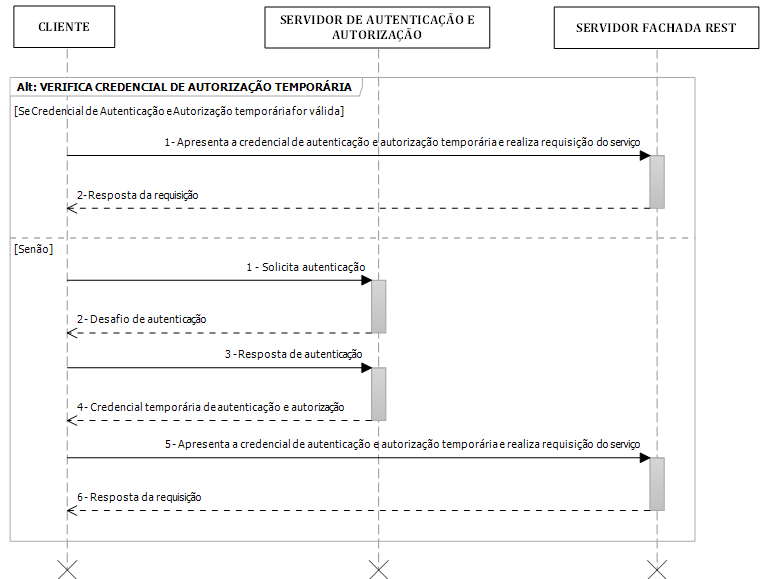
\includegraphics[width=0.8\textwidth]{cenario2_autenticacao.png}
%     \caption{Fluxo do protocolo de autenticação/autorização proposto, 2º cenário.}
%     \label{fig:cenario2}
%\end{figure}


\section{Formalização do protocolo}

O uso de especifica\c c\~{o}es formais na área de criptografia (em particular para especificar protocolos criptogr\'{a}ficos) 
não é recente. Parte dos trabalhos nesta área foram desenvolvidos ainda na década de 90~\cite{Meadows95}, 
possibilitando uma análise mais detalhada dos protocolos. Com isso, o principal objetivo 
tem sido a verifica\c c\~{a}o dos objetivos de seguran\c ca propostos 
pelos autores dos protocolos criptogr\'{a}ficos são alcançados.

Neste trabalho, o protocolo proposto foi descrito formalmente utilizando a lógica BAN, 
com o intuito de favorecer uma melhor comunicação e entendimento utilizando uma linguagem mais precisa. 
Além disso, a propriedade de terminação com a geração da credencial temporária de autenticação e autorização 
foi verificada com um programa escrito em Prolog (ver {\color{red}Anexo~\ref{}}.)


\subsection{Lógica BAN}

A lógica BAN foi desenvolvida por Burrows, Abadi e Needham em 1989, tendo alcan\c cado 
certa popularidade para a análise de confian\c ca e de conhecimento entre os participantes 
dos protocolos criptográficos~\cite{Burrows1990}. BAN \'{e} uma l\'{o}gica pioneira na especifica\c c\~{a}o de 
 protocolos criptográficos, em particular protocolos usados na autenticação e 
distribuição de chaves~\cite{Burrows1990}.

\subsubsection{Notação básica}

Na lógica BAN, existem vários tipos distintos de objetos tais como entidades ou partes que se 
comunicam, chaves de criptografia e fórmulas lógicas. Uma fórmula lógica é uma versão idealizada da mensagem original, 
sendo usualmente referenciada como uma declaração lógica. Em geral, os símbolos $A$, $B$ e $S$ denotam 
entidades ou participantes; $Kab$, $Kas$ e $Kbs$ denotam chaves compartilhadas; $Ka$, $Kb$ e $Ks$ 
denotam chaves públicas e $Ka^{-1}$, $Kb^{-1}$ e $Ks^{-1}$ denotam as chaves privadas dos participantes. 
Finalmente, $Na$, $Nb$ e $Ns$ são os identificadores gerados pelos participantes (referenciados como \emph{nonces} 
na literatura). As construções usadas com maior frequ\^{e}ncia 
são apresentadas na Tabela~\ref{tab:notacaobasicaBAN}:

 \newcommand{\RHQuery}{\textbf{[???]}}
\newcommand{\RHRemark}[1]{\textbf{[#1]}}
\newcommand{\Believess}[2]{{#1}\mathrel{\textbf{\mid\equiv}}{#2}}
\newcommand{\Seess}[2]{{#1}\mathrel{\textbf{\triangleleft}}{#2}}
\newcommand{\Saids}[2]{{#1}\mathrel{\textbf{\mid\sim}}{#2}}

\newcommand{\Believes}[2]{{#1}\mathrel{\textbf{acredita}}{#2}}
\newcommand{\Sees}[2]{{#1}\mathrel{\textbf{recebeu}}{#2}}
\newcommand{\Said}[2]{{#1}\mathrel{\textbf{disse}}{#2}}
\newcommand{\Controls}[2]{{#1}\mathrel{\textbf{controla}}{#2}}
\newcommand{\Fresh}[1]{{#1}\,\textbf{novo}}
\newcommand{\Share}[3]{{#1}\stackrel{#2}{\longleftrightarrow}{#3}}
\newcommand{\ShareSecret}[3]{{#1}\stackrel{#2}{\rightleftharpoons}{#3}}
\newcommand{\PubKey}[2]{{}\stackrel{#1}{\mapsto}{#2}}
\newcommand{\Secret}[3]{{#1}\stackrel{#2}{\leftrightharpoons}{#3}}
\newcommand{\Encrypt}[2]{\{\,{#1}\,\}_{#2}}
\newcommand{\EncryptFrom}[3]{\{\,{#1}\,\}_{#2}^{#3}}
\newcommand{\Attach}[2]{\langle {#1}\rangle_{#2}}

%  \begin{tabular}{cp{16cm}}
\begin{table}[h]
\begin{center}
    \begin{tabular}{|l|p{10cm}|}
    \hline
    \textbf{\emph{Expressão }}         & \textbf{\emph{Leitura/Significado}}                                                                               \\ \hline
    ${P}\mid\equiv{X}$               & $\Believes{P}{X}$: $P$ confia em $X$, ou $P$ acredita que $X$ é verdadeiro. \\ \hline
    
    ${P}\triangleleft{X}$            & $\Sees{P}{X}$: Alguém enviou uma mensagem para $P$ contendo $X$; ou seja, $P$ recebeu $X$.   \\ \hline
    
     ${P}\mid\sim{X}$                 & $\Said{P}{X}$: $P$ alguma vez compartilhou $X$. Pode-se assumir que a entidade $P$ 
        em algum momento enviou uma mensagem incluíndo a declaração $X$.\\ \hline
    
    ${P}\Rightarrow {X}$                 & $\Controls{P}{X}$: $P$ tem jurisdição sobre $X$, onde $P$ é uma autoridade sobre $X$ e deve ser confiável. \\ \hline

    \#(X)                            & novo$(X)$: a fórmula $X$ não foi usada em mensagens anteriores à execução atual do protocolo.  \\ \hline

    $\Share{P}{k}{Q}$                & (lê-se ``k é uma chave satisfatória para $P$ e $Q$''). A chave $k$ n\~{a}o pode ser descoberta 
                                             por qualquer outro participante, exceto $P$, $Q$ ou por alguém que {\color{red}ambos} confiam. \\ \hline

    $\{{X}\}_K$                  & fórmula $X$ foi cifrada com a chave $K$. As mensagens cifradas são legíveis e verificáveis apenas pelos 
                                       participantes que conhecem a chave $K$. \\ \hline

    $\ShareSecret{P}{k}{Q}$         & ${k}$ é um segredo compartilhado entre ${P}$ e ${Q}$ e possivelmente as entidades de confiança de $P$ e $Q$. 
                                                 Somente ${P}$ e ${Q}$ podem usar $k$ para provar suas identidades. \\ \hline
    
    $\PubKey{K}{P}$:               & ${k}$ é a chave pública de ${P}$.  \\ \hline
    \end{tabular}
    \caption {Notação básica da Lógica BAN, adaptação de ~\cite{Burrows1990}.}
\label{tab:notacaobasicaBAN}
\end{center}
\end{table}


\subsubsection{Postulados lógicos}

No estudo de protocolos de segurança é importante diferenciar o tempo das demonstrações ou eventos.  
Caso isso não seja observado, problemas como a não detecção  do  reenvio de mensagens podem 
ocorrer. Dessa forma, a lógica BAN trata dessa distinção dividindo-a em duas épocas: 
presente, que é o tempo durante a execução do protocolo, e o passado,  que refere-se às mensagens enviadas antes da execução do protocolo, 
o que faz com que elas sejam rejeitadas, uma vez que não são confiáveis~\cite{Burrows1990}. 
Essa divisão de tempo é suficiente para facilitar o entendimento sobre como a lógica pode ser manipulada.
Para realizar a análise dos protocolos de segurança, a lógica BAN possui uma s\'{e}rie de postulados lógicos. 
No restante dessa se\c c\~{a}o apresentamos alguns desses postulados, refor\c cando que maiores detalhes 
podem ser encontrados no artigo que introduziu a nota\c c\~{a}o BAN~\cite{Burrows1990}

\begin{enumerate}[(P1)]

 \item Regra de significado da mensagem. Esta regra faz parte da interpretação das mensagens. 
    Para as chaves secretas compartilhadas, temos que

    \begin{displaymath}
        \infer
        {{P}\mid\equiv{{Q}\mid\sim{X}}}
        {{P}\mid\equiv{\Share{P}{k}{Q}}& {P}\triangleleft{\Encrypt{X}{k}}}
        %{\Believes{P}{\Said{Q}{X}}}
        %{\Believes{P}{\Share{P}{k}{Q,}}&\Sees{P}{\Encrypt{X}{k}}}
    \end{displaymath}

Ou seja, assumindo que $P$ acredita que $k$ é uma chave satisfatória para se comunicar com $Q$, e que 
$P$ recebeu a mensagem $X$ cifrada com a chave $k$, então $P$ acredita que $Q$ uma vez disse $X$. 
De forma similar, esse postulado quando consideramos chaves p\'{u}blicas estabelece que

    \begin{displaymath}
        \infer
        {{P}\mid\equiv{{Q}\mid\sim{X}}}
        {{P}\mid\equiv{\PubKey{K}{Q}}& {P}\triangleleft{\Encrypt{X}{k ^{-1}}}}
                %{\Believes{P}{\Said{Q}{X}}}
                %{\Believes{P}{\Share{P}{k}{Q,}}&\Sees{P}{\Encrypt{X}{k}}}
    \end{displaymath}



\item Regra de verificação do identificador. Essa regra estabelece que, dada uma mensagem recente, 
enviada durante a execução atual do protocolo, \'{e} \'{e} poss\'{i}vel 
assumir que o emissor confia na mensagem.

  \begin{displaymath}
    \infer
    {{P}\mid\equiv{{Q}\mid\equiv{X}}}
    {{P}\mid\equiv{\#(X),}& {P}\mid\equiv{{Q}\mid\sim{X}}}
    %{\Believes{P}{\Believes{Q}{X}}}
    %{\Believes{P} novo$(X),$ &\Believes{P}{\Said{Q}{X}}}
  \end{displaymath}

   Se $P$ acredita que $X$ é novo e $P$ acredita que em algum momento $Q$ disse $X$, então $P$ assume que $Q$ confia em X.

\item Regra da jurisdição. Esta regra representa a confiança e a autoridade de uma entidade sobre as declarações.
\begin{displaymath}
    \infer
    {{P}\mid\equiv{X}}
    {{P}\mid\equiv{{Q}\Rightarrow {X},}& {P}\mid\equiv{{Q}\mid\equiv{X}}}
   % {\Believes{P}{X}}
   % {\Believes{P}{\Controls{Q}{X},} &\Believes{P}{\Believes{Q}{X}}}
  \end{displaymath}

   Se $P$  acredita que $Q$ tem jurisdição sobre a declaração $X$ e $P$ acredita que $Q$ acredita em $X$, então $P$ confia na declaração $X$.

\end{enumerate}

Estes são os postulados fundamentais na análise formal do protocolo criptográfico proposto nessa disserta\c c\~{a}o. 
A utilização destas regras, juntamente com as notações descritas na sessão anterior, possibilita 
o estabelecimento da confian\c ca entre os participantes de um protocolo.

\subsection{Análise formal do protocolo proposto}

Nesta sessão apresentamos a análise formal do protocolo de autenticação e autorização proposto, seguindo o processo 
descrito em~\cite{Burrows1990}. De acordo com o referido processo, a an\'{a}lise de um protocolo é realizada em quatro etapas, que serviram para 
organizar o restante dessa se\c c\~{a}o. 

\subsubsection{Idealização do protocolo}

\newcommand{\HT}[3]{\{\,{#1}\,\}\,{#2}\,\{\,{#3}\,\}}
\newcommand{\Msg}[3]{{#1}\longrightarrow{#2}:\,{#3}}

Para especificar o protocolo formalmente, foram utilizadas algumas notações para representar os elementos participantes. Logo, os símbolos ${A}$, ${B}$ e ${C}$ são utilizadas para representar respectivamente as entidades que trocam mensagens entre si. No protocolo proposto, temos como participantes os n\'{o}s Cliente, \servidorRest{} e 
\servidorAA. As chaves públicas das entidades ${A}$, ${B}$ e ${C}$ são representadas, respectivamente, por ${Ka}$, ${Kb}$ e ${Kc}$. As chaves privadas, seguindo o mesmo pressuposto, são representadas pelos símbolos ${{Ka}^{-1}}$, ${{Kb} ^{-1}}$ e ${{Kc} ^{-1}}$. Os elementos ${Cred_A}$ e ${Cod_{Srv_A}}$ representam, respectivamente, 
a credencial utilizada pela entidade ${A}$ e o código que identifica o serviço que a entidade ${A}$ deseja consumir.

O desafio, gerado pela entidade ${C}$ e enviado a entidade ${A}$, \'{e} representado pela fórmula ${N_{CA}}$. Essa f\'{o}rmula contempla o código do desafio gerado pela entidade ${C}$ e 
o código da credencial aleatória da entidade ${A}$. A resposta do desafio gerada pela entidade ${C}$ e enviada à entidade ${A}$ é representada pela 
f\'{o}rmula ${Resp_{AC}}$. Essa f\'{o}rmula corresponde ao código do desafio gerado pela entidade ${C}$ e a credencial solicitada pela entidade ${A}$. 
${Ts_A}$ e ${Ts_C}$ são, respectivamente, os \emph{timestamps} emitidos pelas entidades ${A}$ e ${C}$.

O símbolo ${Msg_{AC}}$ representa o resumo da mensagem enviada pela entidade ${A}$ \`{a} entidade ${C}$,  ${Msg_{CA}}$ representa o resumo da mensagem enviada pela entidade ${C}$ 
\`{a} entidade ${A}$ e ${Msg_{AB}}$ representa o resumo da mensagem enviada pela entidade ${A}$ \`{a} entidade ${B}$. O elemento ${H}$ representa a aplica\c c\~{a}o de 
uma fun\c c\~{a}o \emph{HASH} a uma mensagem.\footnote{Na implementa\c c\~{a}o do protocolo, foi utilizado o algoritmo SHA3}
Finalmente, o símbolo ${Exp_A}$ representa a data/hora  de expiração da credencial temporária de autorização e autenticação, ${C_{Aut}}$ corresponde à credencial temporária de autorização e autenticação gerada para a entidade A e ${Req_A}$ refere-se à requisição de serviços realizadas a partir da entidade $A$;
utilizando algum dos m\'{e}todos do protocolo HTTP (GET, PUT, POST ou DELETE).

Para especificar formalmente um protocolo de segurança utilizando a lógica BAN, é necessário idealizar o protocolo e, a partir da aplicação dos postulados e das suposições iniciais, verificar se ele atinge ou não o seu objetivo. A idealização do protocolo proposto \'{e} descrito na figura~\ref{fig:protocoidealizado}, representando o fluxo de troca de mensagens executado pelo protocolo. {\color{blue}n\~{a}o entendi: Todas as mensagens são consideradas na análise, pois utilizam criptografia assimétrica desde a primeira troca de mensagens}.

\begin{figure}[!htb]
    \centering
    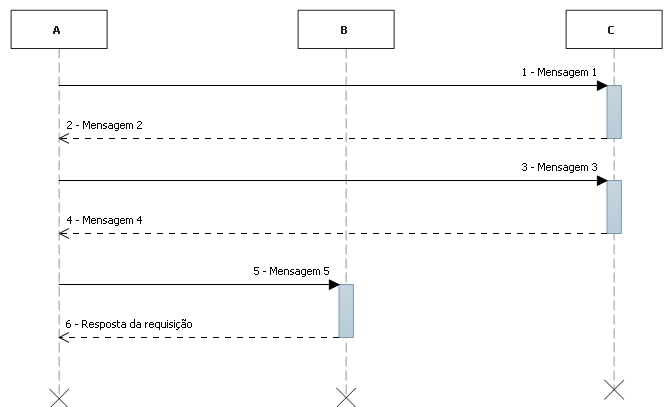
\includegraphics[width=0.8\textwidth]{fluxo_autenticacao_BAN.png}
    \caption{Diagrama com a idealização do protocolo de autenticação/autorização proposto}
    \label{fig:protocoidealizado}
\end{figure}

\begin{enumerate}
  \item Mensagem 1: $\Msg{A}{C}{\Encrypt{Ts_A,Cred_A,H{\Encrypt{Msg_{AC}}{Ka ^{-1}}}}{Kc}}$.
  \item Mensagem 2: $\Msg{C}{A}{\Encrypt{Ts_C,{N_{CA}},H{\Encrypt{Msg_{CA}}{Kc ^{-1}}}}{Ka}}$.
  \item Mensagem 3: $\Msg{A}{C}{\Encrypt{Ts_A,{Resp_{AC}},Cod_{Srv_A},H{\Encrypt{Msg_{AC}}{Ka ^{-1}}}}{Kc}}$.
  \item Mensagem 4: $\Msg{C}{A}{\Encrypt{Ts_C,Exp_A,\#(\ShareSecret{A}{{C_{Aut}}}{C}),H{\Encrypt{Msg_{CA}}{Kc ^{-1}}}}{Ka}}$.
  {\color{blue}\item Mensagem 5: $\Msg{A}{B}{\Encrypt{Ts_A,(\ShareSecret{A}{{C_{Aut}}}{C}),H{\Encrypt{Msg_{AB}}{Ka ^{-1}}}}{Ka}},{Req_A}$.}\footnote{V\'{a}rias d\'{u}vidas. Por que enviar 
$Req_A$? Por que essa mensagem para B?} 
\end{enumerate}

\subsubsection{Suposições}\label{sec:Suposicoes}

O objetivo do protocolo é fazer com que a entidade ${A}$ seja autenticada pela entidade ${C}$ e obtenha uma credencial de autenticação e autorização temporária, referente a uma requisição de um serviço que a entidade ${A}$ deseja consumir. Com isso, a credencial de autenticação e autorização temporária pode ser utilizada pela entidade ${A}$ no momento da requisição do serviço \`{a} entidade ${B}$ e, assim, realizar a computa\c c\~{a}o que deseja via o consumo a um servi\c co de forma segura. Para isso, algumas suposições iniciais são estabelecidas e, juntamente com a aplicação  dos postulados da lógica BAN, busca-se verificar se o protocolo alcan\c ca o objetivo proposto. Todas as suposições, apresentadas na Tabela~\ref{tab:suposicoesBAN}, são baseadas no uso de um canal seguro de comunicação SSL/TSL; onde tanto o receptor  quanto o emissor do serviço são conhecidos e 
autenticados {\color{blue}isso eh necess\'{a}rio indicar?} com o uso de certificados digitais X.509.

\begin{table}[h]
\begin{tabular}{cllcl}
\textbf{Suposição} & \textbf{Descrição} &  & \textbf{Suposição} & \textbf{Descrição} \\
\textbf{1 -}       & $ A \mid\equiv$  ${\PubKey{Kc}{C}}$                 &  & \textbf{9 -}       & $ B \mid\equiv$ $ C \Rightarrow $ $\#(\ShareSecret{A}{{C_{Aut}}}{C})$ \\
\textbf{2 -}       & $ B \mid\equiv$  ${\PubKey{Ka}{A}}$                 &  & \textbf{10 -}      & $ A \mid\equiv$ $ C \mid\equiv $ $\#(\ShareSecret{A}{{C_{Aut}}}{C})$ \\
\textbf{3 -}       & $ C \mid\equiv$  ${\PubKey{Ka}{A}}$                 &  & \textbf{11 -}      & $ B \mid\equiv$ $ C \mid\equiv $ $\#(\ShareSecret{A}{{C_{Aut}}}{C})$ \\

\textbf{4 -}       & $ A \mid\equiv$  $\#{Ts_C}$                         &  & \textbf{12 -}      & $ A \mid\equiv$  $\#(\ShareSecret{A}{{C_{Aut}}}{C})$  \\

\textbf{5 -}       & $ B \mid\equiv$  $\#{Ts_A}$                         &  & \textbf{13 - }      & $ B \mid\equiv$  $\#(\ShareSecret{A}{{C_{Aut}}}{C})$  \\

\textbf{6 -}       & $ C \mid\equiv$  $\#{Ts_A}$                         &  & \textbf{ }                    &                                      \\
\textbf{7 -}       & $ A \mid\equiv$  ${Exp_A}$                          &  & \textbf{ }                   &
\\
\textbf{8 -}       & $ A \mid\equiv$  $ C \Rightarrow $ $\#(\ShareSecret{A}{{C_{Aut}}}{C})$   &   & \textbf{ }     &                               \\
\end{tabular}
\caption {Suposições aplicadas ao protocolo proposto.}
\label{tab:suposicoesBAN}
\end{table}


Dessa forma, temos que as suposições 1, 2 e 3 garantem que as entidades participantes ${A}$, ${B}$ e ${C}$ confiam  nas chaves públicas das entidades que farão as trocas de mensagem. As suposições 4, 5 e 6 são \emph{timestamps}, o que denota que as entidades ${A}$, ${B}$ e ${C}$ devem estar sincronizadas. Sendo assim, a entidade ${A}$ acredita que o \emph{timestamp} ${Ts_C}$ é novo e foi gerado recentemente. Da mesma forma que as entidades ${B}$ e ${C}$ acreditam  que o \emph{timestamp} ${Ts_A}$ também é novo e foi gerado recentemente. A suposição 7 é utilizada pela entidade ${A}$ para garantir que a credencial de autenticação e autorização gerado pela entidade ${C}$ não expirou e que pode ser utilizada. As suposições 8 e 9 denotam que as entidades ${A}$ e ${B}$ acreditam que entidade ${C}$ tem jurisdição  sobre a credencial de autenticação e autorização gerada. Portanto, as suposições 10 e 11 garantem que as entidades ${A}$, ${B}$ acreditam que a credencial de autenticação e autorização gerada é nova é foi realmente gerada pela entidade ${C}$. Finalmente, as suposições 12 e 13 garantem que as entidades ${A}$ e ${B}$ acreditam na nova credencial de autenticação e autorização temporária representada por ${C_{Aut}}$.

\subsubsection{Provas}

Como o objetivo final do protocolo é autenticar a entidade ${A}$, de forma que ela obtenha uma credencial de autenticação e autorização temporária e referente a uma requisição de serviço desejado. Nessa se\c c\~{a}o, será realizada uma análise de cada mensagem do protocolo idealizado, aplicando os postulados lógicos e suposições com 
o intuito de provar que o protocolo consegue atingir o objetivo proposto.

Na primeira mensagem, a entidade ${A}$ envia sua credencial, um \emph{timestamp} e o código do serviço que ele está querendo consumir ao \servidorAA, 
representado pela entidade ${C}$. A mensagem enviada é assinada com a chave privada do participante ${A}$  e cifrada com a chave pública do participante ${C}$. 
Ap\'{o}s o recebimento dessa mensagem, o estado da execu\c c\~{a}o do protocolo evolui conforme a descri\c c\~{a}o

\textbf{Mensagem 1}: $\Msg{A}{C}{\Encrypt{Ts_A,Cred_A,H{\Encrypt{Msg_{AC}}{Ka ^{-1}}}}{Kc}}$.

$C\triangleleft$ ${\Encrypt{Ts_A,Cred_A,Cod_{Srv_A},H{\Encrypt{Msg_{AC}}{Ka ^{-1}}}}{Kc}}$

$C\mid\equiv A \mid\sim $  $H\{Msg_{AC}\}$

$C\mid\equiv A \mid\sim$ ${\#Ts_A}$

$C\mid\equiv$ ${Cred_A,Cod_{Srv_A}}$

Dessa forma, $C$ recebe a fórmula ${\Encrypt{Ts_A,Cred_A,Cod_{Srv_A},H{\Encrypt{Msg_{AC}}{Ka ^{-1}}}}{Kc}}$ e, usando sua chave privada, decifra a fórmula recebida. 
Após decifrar a fórmula, e aplicando a regra do significado da mensagem na suposição 3 e usando a função $H \{Msg_{AC}\}$ confirma a autenticidade e integridade da mensagem. 
Por fim, aplica a regra de verificação do identificador na suposição 6 usando a fórmula ${Ts_A}$ para obter a credencial da entidade ${A}$ (identificada pela 
f\'{o}rmula ${Cred_A}$). 

Na segunda mensagem, após receber e validar os dados enviados por $A$, a entidade ${C}$ gera um desafio de autenticação, ${N_{CA}}$. O desafio consiste em fazer uma busca aleatória à tabela de credenciais e selecionar um código de credencial que esteja associado \`{a} entidade $A$. Em seguida grava-se o desafio, a data e hora de geração do desafio e a resposta esperada em uma base de dados. Na sequência, uma mensagem \'{e} enviada uma mensagem \'{a} entidade $A$. Tal mensagem, que contem 
o desafio e um \emph{timestamp}, precisa ser assinada com a chave privada da entidade ${C}$ e cifrada com a chave pública da entidade ${A}$. 
Logo, temos que:

\textbf{Mensagem 2}: $\Msg{C}{A}{\Encrypt{Ts_C,{N_{CA}},H{\Encrypt{Msg_{CA}}{Kc ^{-1}}}}{Ka}}$.

$A \triangleleft$ ${\Encrypt{Ts_C,{N_{CA}},H{\Encrypt{Msg_{CA}}{Kc ^{-1}}}}{Ka}}$

$A \mid\equiv C \mid\sim $  $H \{Msg_{CA}\}$

$A \mid\equiv C \mid\sim$ ${Ts_C}$

$A \mid\equiv$ ${N_{CA}}$

A entidade $A$ recebe a fórmula ${\Encrypt{Ts_C,{N_{CA}},H{\Encrypt{Msg_{CA}}{Kc ^{-1}}}}{Ka}}$ e a decifra usando sua chave privada. Em seguida, aplicando a regra do significado da mensagem na suposição 1 usando a função $H \{Msg_{CA}\}$, confirma a autenticidade e integridade da mensagem. Por fim, aplica a regra de verificação do identificador na suposição 4, usando a fórmula ${Ts_C}$ para obter o desafio ${N_{CA}}$ gerado pela entidade ${C}$. Como resultado, ${A}$ obtém  o desafio de autenticação gerado pela entidade ${C}$.

Na terceira mensagem, a entidade ${A}$, após receber e validar o desafio gerado pela entidade ${C}$, envia a resposta ${Resp_{AC}}$, conforme solicitado. Essa resposta consiste em informar o código do desafio gerado pela entidade ${C}$ e a credencial associada ao código de credencial solicitada pela entidade ${C}$. Além disso, a entidade ${A}$ deve informar o código do serviço que deseja consumir. Dessa forma, temos:

\textbf{Mensagem 3}: $\Msg{A}{C}{\Encrypt{Ts_A,{Resp_{AC}},Cod_{Srv_A},H{\Encrypt{Msg_{AC}}{Ka ^{-1}}}}{Kc}}$.

$C\triangleleft$ ${\Encrypt{Ts_A,{Resp_{AC}},H{\Encrypt{Msg_{AC}}{Ka ^{-1}}}}{Kc}}$

$C\mid\equiv A \mid\sim $  $H \{Msg_{AC}\}$

$C\mid\equiv A \mid\sim$ ${\#Ts_A}$

$C\mid\equiv$ ${Resp_{AC}}$

A entidade $C$ recebe a fórmula ${\Encrypt{Ts_A,{Resp_{AC}},H{\Encrypt{Msg_{AC}}{Ka ^{-1}}}}{Kc}}$ e a decifra usando sua chave privada. Em seguida, aplicando a regra do significado da mensagem na suposição 3 e usando a função $H \{Msg_{AC}\}$, confirma a autenticidade e integridade da mensagem. Por fim, aplica a regra de verificação do identificador na suposição 6 usando a fórmula ${Ts_A}$ para obter os dados da resposta do desafio ${Resp_{AC}}$. Com isso, \'{e} poss\'{i}vel 
validar a resposta enviada e autenticar a entidade ${A}$, dando início ao processo de autorização. Como resultado temos que a entidade ${C}$ autentica a entidade ${A}$.

Na mensagem 4, após autenticar a entidade ${A}$, a entidade ${C}$ procede com o processo de autorização, que consiste em verificar qual serviço a entidade está querendo consumir. 
Para isso, a entidade C verifica o código de serviço solicitado pela entidade ${A}$, $Cod_{Srv_A}$, que foi informado no envio da mensagem 3. Se a entidade ${A}$ possuir os 
privilégios necessários para consumir o serviço requisitado, a entidade ${C}$ gera uma nova credencial de autorização temporária para o serviço solicitado. Em seguida, 
a entidade ${C}$ grava a credencial ${(\ShareSecret{A}{{C_{Aut}}}{C})}$, o código do serviço que a entidade ${A}$ está requerendo, a data e hora de criação, a data de expiração e o código do contrato da entidade ${A}$. Terminado esse procedimento, a entidade ${C}$, envia uma mensagem contendo a credencial ${(\ShareSecret{A}{{C_{Aut}}}{C})}$, a data e hora de expiração da credencial (${Exp_A}$) e um \emph{timestamp} a entidade ${A}$. Esta mensagem é assinada com a chave privada da entidade ${C}$ e cifrada com a chave 
pública da entidade ${A}$. 


\textbf{Mensagem 4}: $\Msg{C}{A}{\Encrypt{Ts_C,Exp_A,\#(\ShareSecret{A}{{C_{Aut}}}{C}),H{\Encrypt{Msg_{CA}}{Kc ^{-1}}}}{Ka}}$.

$A \triangleleft$ $\Msg{C}{A}{\Encrypt{Ts_C,Exp_A,\#(\ShareSecret{A}{{C_{Aut}}}{C}),H{\Encrypt{Msg_{CA}}{Kc ^{-1}}}}{Ka}}$.

$A \mid\equiv C \mid\sim $  $H \{Msg_{CA}\}$

$ A \mid\equiv C \mid\sim$ ${Ts_C}$

$A \mid\equiv C \mid\sim$ ${Exp_A}$

$A \mid\equiv C \Rightarrow $  ${\#(\ShareSecret{A}{{C_{Aut}}}{C})}$

$A \mid\equiv C \mid\equiv $  ${\#(\ShareSecret{A}{{C_{Aut}}}{C})}$

$A \mid\equiv$ ${\#(\ShareSecret{A}{{C_{Aut}}}{C})}$

A entidade ${A}$ recebe a fórmula ${\Encrypt{Ts_C,Exp_A,\#(\ShareSecret{A}{{C_{Aut}}}{C}),H{\Encrypt{Msg_{CA}}{Kc ^{-1}}}}{Ka}}$ e a decifra usando sua chave privada. Em seguida, aplicando a regra do significado da mensagem na suposição 1 e usando a função $H \{Msg_{CA}\}$, confirma a autenticidade e integridade da mensagem. A entidade $A$ 
aplica a regra de verificação do identificador nas suposições 4 e 7 usando as fórmulas ${Ts_C}$  e ${Exp_A}$. E, finalmente, aplicando a regra da jurisdição, nas suposições 7 e 9, obtém a credencial de autorização temporária ${\#(\ShareSecret{A}{{C_{Aut}}}{C})}$.

Finalmente, na quinta mensagem, a entidade ${A}$ após receber e validar a mensagem enviada pela entidade ${C}$, obtendo assim a credencial de autenticação e autorização temporária, ${\#(\ShareSecret{A}{{C_{Aut}}}{C})}$, envia uma mensagem \`{a} entidade ${B}$ contendo a requisição do serviço que deseja consumir juntamente com a credencial de autorização temporária. Esta mensagem é assinada com a chave privada da entidade ${A}$ e cifrada com a chave pública da entidade ${B}$. 

\textbf{Mensagem 5}: $\Msg{A}{B}{\Encrypt{Ts_A,(\ShareSecret{A}{{C_{Aut}}}{C}),H{\Encrypt{Msg_{AB}}{Ka ^{-1}}}}{Kb}},{Req_A}$.

$B\triangleleft$  ${\Encrypt{Ts_A,(\ShareSecret{A}{{C_{Aut}}}{C}),H{\Encrypt{Msg_{AB}}{Ka ^{-1}}}}{Kb}},{Req_A}$

$B\mid\equiv A \mid\sim $  $H\{Msg_{AB}\}$

$B\mid\equiv A \mid\sim$ ${Ts_A}$

$B\mid\equiv A \Rightarrow $  ${\#(\ShareSecret{A}{{C_{Aut}}}{C})}$

$B\mid\equiv A \mid\equiv $  ${\#(\ShareSecret{A}{{C_{Aut}}}{C})}$

$B\mid\equiv$ ${\#(\ShareSecret{A}{{C_{Aut}}}{C})}$

Como resultado, a entidade $B$ recebe a fórmula ${\Encrypt{Ts_A,(\ShareSecret{A}{{C_{Aut}}}{C}),H{\Encrypt{Msg_{AB}}{Ka ^{-1}}}}{Kb}},{Req_A}$, e a decifra, usando sua chave privada. Em seguida, aplicando a regra do significado da mensagem na suposição 2 e usando a função $H\{Msg_{AB}\}$, confirma a autenticidade e integridade da mensagem. A entidade $B$ aplica a regra de verificação do identificador na suposições 5 usando as fórmulas ${Ts_A}$. Finalmente, aplicando a regra da jurisdição nas suposições 8 e 10, obtém a credencial de autorização temporária ${\#(\ShareSecret{A}{{C_{Aut}}}{C})}$ e autoriza a entidade A a consumir a requisição ${Req_A}$. Como resultado, 
${B}$ autoriza ${A}$, a partir da nova credencial ${(\ShareSecret{A}{{C_{Aut}}}{C})}$, a consumir a requisição ${Req_A}$

\subsubsection{Análise}

A análise demonstra que o protocolo de autenticação e autorização proposto alcança os objetivos apresentados--- ou seja, a autenticação da entidade ${A}$ e a emissão da credencial de autenticação e autorização temporária. Isso permite que a entidade ${A}$ consuma o serviço requerido. É importante frisar que a lógica BAN foi utilizada para (a) comunicar 
de forma mais precisa a execução do protocolo e (b) permitir uma verifica\c c\~{a}o mais precisa sobre possíveis falhas no protocolo.
{\color{blue}precisamos discutir isso, pois voc\^{e} apresenta uma an\'{a}lise de seguran\c ca no pr\'{o}ximo cap\'{i}tulo} Para verificar a segurança do protocolo é necessário que seja empregado um método de criptoanálise sobre a criptografia utilizada e assim verificar quais são vulnerabilidades que o protocolo ou os algoritmos criptográficos empregados estão sujeitos.


\section{Implementação}\label{sec:implementacao}

Após a definição do protocolo proposto, e para atender o interesse na realização de testes de desempenho que objetivam avaliar o impacto da solução, 
foi feita a implementa\c c\~{a}o de um protótipo para o protocolo de autenticação e autorização. Esse protótipo foi desenvolvido em conjunto com um 
trabalho de conclus\~{a}o de curso do aluno Alexandre Lucchesi (da Engenharia da Computa\c c\~{a}o, UnB).

\subsection{Protótipo}

Para implementar o protótipo do protocolo proposto foi necessário desenvolver cada um dos componentes (Cliente, \servidorAA e \servidorRest) descritos na arquitetura 
do protocolo na seção~\ref{sec:ArqProtocolo}. Para isso, foi utilizada a linguagem de programação funcional Haskell, com o compilador GHC (Glasgow Haskell Compiler). 
Para o controle de dependências e gerenciamento de \emph{build} de aplicações foi utilizada a ferramenta Cabal, que é um o gerenciador de pacotes do Haskell. Com ele é possível construir aplicações e bibliotecas de forma padronizada, organizada e portável. Para criar o protótipo ainda foi utilizado o framework Haskell para desenvolvimento web, denominado Snap \emph{Framework} que é necessário para lidar com as requisições HTTP. Tais requisi\c c\~{o}es são utilizadas pelo protocolo de autenticação e autorização proposto. Além disso, foi utilizado o HsOpenSSL que é um OpenSSL {\color{red}vinculativo} para Haskell, utilizado para garantir a utilização do HTTPS em todas as trocas de mensagem a partir de código Haskell.

Para a assinatura digital das mensagens utilizadas pelo protocolo foi utilizado o algoritmo RSASSA\-PKCS\-v1\_5 SHA\-256 conforme orientação descrita na publicação~\cite{ietfjws} e para criptografia foi utilizado o algoritmo de criptografia assimétrica, RSAES\-PKCS1\-V1\_5, para cifrar a chave simétrica utilizada no algoritmo de criptografia simétrica AES\_128\_CBC\_HMAC\_SHA\_256 que foi utilizado para cifrar a mensagem. Procurou-se seguir a orientação do que é preconizado na publicação~\cite{jwt2014}.

O servidor de banco de dados foi implementado utilizando o banco de dados não relacional \emph{Apache CouchDB}, que é um banco de dados flexível e tolerante a falhas que usa \emph{JSON} para armazenar os dados e JavaScript como sua linguagem de consulta usando o MapReduce. Além disso, o \emph{Apache CouchDB} 
oferece uma API de acesso de acordo com o estilo REST.

O protótipo implementado não objetivou a otimização de c\'{o}digo. Seu objetivo foi o de possibilitar a realização dos testes de desempenho em uma configura\c c\~{a}o 
mais rudimentar em termos de desempenho, o que leva a possibilidades de melhoria em rela\c c\~{a}o ao processamento das requisi\c c\~{o}es. 
Al\'{e}m disso, o prot\'{o}tipo permitiu verificar as funcionalidades do protocolo proposto.


\section{Síntese do capítulo}

Este capítulo apresentou os requisitos e a arquitetura do protocolo de autenticação e autorização proposto. Além disso,  o capítulo apresentou a formalização do protocolo utilizando à lógica BAN. Finalmente, foi apresentada de forma sucinta a implementação de um protótipo para p protocolo proposto. No próximo capítulo fazemos uma 
análise de seguran\c ca do protocolo proposto 
(conforme o trabalho apresentado em~\cite{traust08}) e apresentamos uma an\'{a}lise de 
desempenho a fim de mensurar o impacto do protocolo {\color{red}n\~{a}o sei se o impacto \'{e}} 
na infraestrutura da PCDF. 
